\documentclass[12pt, onecolumn]{article}
\usepackage{times}
\usepackage{graphicx}
\usepackage{anyfontsize}
\usepackage{makecell}
\usepackage[linesnumbered, ruled, vlined]{algorithm2e}
\SetAlFnt{\small}
\SetAlCapFnt{\large}
\SetAlCapNameFnt{\large}




% Keywords command
\providecommand{\keywords}[1]
{
  \small	
  \textbf{\textit{Keywords---}} #1
}

\title{Edge-Adaptable Serverless Acceleration for Machine Learning IoT Applications}
\author{Michael Zhang, Chandra Krintz, and  Rich Wolski \\
        \small Dept. of Computer Science \\
        \small Univ. of California, Santa Barbara \\
        \small \{lebo, ckrintz, rich\}@cs.ucsb.edu \\
}
\date{} % Comment this line to show today's date


\hyphenation{multi-university}

\newcommand{\ignore}[1]{}


\begin{document}
\maketitle

\begin{abstract}
\label{sec:abstract}
Serverless computing is an emerging event-driven programming model that accelerates the development and deployment of scalable web services on cloud computing systems. Though widely integrated in the public cloud, serverless computing 
use is nascent for edge-based, IoT deployments.

In this work, we present STOIC (Serverless TeleOperable HybrId Cloud), an IoT application deployment and offloading system that extends the serverless model in three ways. First, STOIC adopts a dynamic feedback control mechanism to precisely predict latency and dispatch workloads uniformly across edge and cloud systems using a distributed serverless framework. Second, STOIC leverages hardware acceleration (e.g. GPU resources) for serverless function execution when available from the underlying cloud system. Third, STOIC can be configured in multiple ways to overcome deployment variability associated with public cloud use. We overview the design and implementation of STOIC and empirically evaluate it using real-world machine learning applications and multi-tier IoT deployments (edge and cloud). Specifically, we show that STOIC can be used for \textit{training} image processing workloads (for object recognition) -- once thought too resource-intensive for edge deployments. We find that STOIC reduces overall execution time (response latency) and achieves placement accuracy that ranges from 92\% to 97\%.

\end{abstract}

\keywords{serverless, IoT, scheduling, cloud functions, GPU}



\section{Introduction}
\label{sec:intro}
Serverless computing (also known as Functions-as-a-Ser\-vice (FaaS))~\cite{ref:aws-lambda,ref:faas3,ref:afunctions-16} is a popular cloud service for hosting and automatically scaling applications. Originally designed for web services~\cite{ref:lambda-webservices,ref:lambda-microservices}, serverless computing defines a simple, event-driven programming model and a platform where developers write simple, short-lived functions that are invoked by the platform in response to specific system-wide events (e.g. storage updates, notifications, messages received, changes in state, custom events, etc.). Serverless platforms automatically configure and provision isolated execution environments (e.g. Linux containers) on-demand and users pay only for the resources their functions use during execution. Given its success to date, other public cloud providers and open source communities have released serverless platforms with similar functionality~\cite{ref:gfunctions-16,ref:openwhisk-16,ref:ironio-16}.

Moreover, serverless computing has been extended to work at the ``edge'' of the network to reduce the response latency and bandwidth associated with public cloud use by data-driven applications (e.g.  those that target the Internet of Things (IoT))~\cite{ aws-greengrass, iothub-web, iotedge-web}. Doing so is challenging however, because there is a scarcity of computing and storage resources at the edge relative to resource-rich public and private clouds. Moreover, public/private clouds may offer specialized hardware (e.g. GPUs) that can significantly speed up machine learning applications, which is not commonly available in resource-restricted edge clouds.

In this paper, we investigate the use of serverless computing across the edge and public cloud deployments (hybrid cloud deployments). We develop a scheduling system, called the Serverless TeleOperable Hybrid Cloud (STOIC), which automatically places and deploys functions across these systems aiming to reduce the total execution time latency (versus using either system in isolation). We specifically target image-based, object recognition using Tensorflow across hybrid deployments in this work.

\iffalse
In particular, we couple edge systems without GPUs with public (shared) cloud systems with GPUs. Moreover, we do so for an important class of machine learning applications -- those that perform model training (versus inference or classifications), given that much past work has argued that training should not be performed at the edge due to limited resources and lack of acceleration~\cite{ref:dependability}.
\fi

STOIC automatically places serverless functions at the edge (without GPUs) or in public cloud instances (equipped with either 1 or 2 GPUs), depending on which assignment it predicts will result in the least user-perceived application latency. We use the system to perform online training and inference for batches of images from motion-triggered, camera traps that capture images of wildlife deployed in a remote location, with little Internet connectivity.

% removed for blind review at Sedgwick Research
%Reserve~\cite{ref:sedgwick}. 

STOIC has two placement scenarios: the first places functions only at the runtime with the least predicted latency, whereas the second places functions concurrently at both edge and public cloud, but then terminates public cloud execution if/when it determines that the edge will finish sooner. The former scenario is called \textit{Selector} mode. The latter scenario, called \textit{Duplicator} mode, is useful when the cloud and/or network performance used for deployment is intermittent or highly variable, or when executing at the edge incurs no cost or other penalty. Serving as a safety net, edge cloud in duplicator mode guarantees a result generated within a reason time frame and cost. Our results show that STOIC speeds up the total response time of the application by 3.3x versus our baseline scenario. In selector mode, STOIC achieves a placement accuracy of 92\% relative to the optimal placement.  In duplicator mode, STOIC accuracy is 95\% for 2 GPUs and 97\% (versus optimal) for 1 GPU cloud deployments over 24 hour.


\iffalse
To do so, STOIC estimates, using execution histories, transfer time (for sending image batches to the public cloud), deployment time (to spin up runtime containers in the public cloud), and execution time (for executing the workloads on the edge and public cloud). The STOIC platform processes the images in batches, performing model training either at an edge cloud deployed locally or on a remote, shared, GPU cloud called Nautilus~\cite{ref:nautilus}.
\fi




In summary, with this paper, we make the following contributions.
\begin{itemize}
\item We design and implement a serverless framework that spans heterogeneous edge and cloud systems, serving IoT requests, and leveraging GPU acceleration;
\item We investigate feedback control mechanism and various analytical methodologies to precisely model the unstable edge and public cloud environments; and 
\item We empirically evaluate the efficacy of using this extended serverless model for machine learning applications and IoT deployments.
\end{itemize}

In the following sections, we present the design and implementation of STOIC. We then present our experimental methodology and empirical evaluation of the system and application workloads, using a distributed serverless deployment (Section~\ref{sec:results}). Finally, we discuss related work (Section~\ref{sec:related}) and present our conclusions and future work plans (Section~\ref{sec:conc}).









\iffalse
In this paper, we present STOIC (Serverless TeleOperable Hybrid Cloud) that embraces such designing philosophy. Unique to STOIC, however, is its offloading system which intelligently places the application workload on edge and cloud systems based on its precise prediction of total latency. We consider three major contributions from this work: (1) we design and implement a serverless framework serving IoT requests by leveraging GPU acceleration. (2) we investigate feedback control mechanism and various analytical methodologies to precisely model the unstable edge and public cloud environments. (3) we test the efficacy of using this extended serverless model for machine learning applications that span edge-cloud systems, and empirically evaluate the performance of doing so. Using real workloads and deployments, 

located near and directly
connected to IoT devices and
sensors~\cite{edge,bonomi2012fog,cloudlets,cloudlets2012satya,verbelen2012cloudlets}.
Example public cloud offerings include AWS Greengrass~\cite{greengrassweb,awsiot-web} and
Azure Iot Edge~\cite{iotedge-web,iothub-web}


These open source Recently, serverless has been shown to be useful for taming the complexity of  popular for IoT applications because it 

FaaS, thus is ideally suited to large-scale, IoT application development because of its simplicity,
asynchronous and event-driven execution model, automated application management at scale,
and low monetary operational cost.

In a monolithic architecture, the application logic is organized in a holistic master piece that is hard for developers to deploy and maintain. The incentives of faster iteration and lightweight execution unit originates the shift to microservices and further serverless computing, in which developers write applications that consist of independent and stateless functions that the cloud invokes on-demand, in response to system-wide events.

Such function-level abstraction also provides fine-grained computational resource isolation and usage, meaning that each serverless function can autoscale independently based on the concurrency of triggering events. Providing this elasticity helps avoid a single point failure and performance bottlenecks in data-intensive application. From this perspective, serverless architecture is an ideal system for online training~\cite{ref:online} and inference applications, which manipulate large amounts of data in batches and execute concurrent applications in a stateless manner.

To enable such an event-driven system, one typical scenario is for machine learning applications that receive their data from heterogeneous IoT devices, ranging from thermostats to Fitbits to autonomous vehicles. For such deployments, application execution should be in the vicinity of the data sources to achieve fast response times. Such settings motivate us to extend the serverless model to the edge for executing data analytics applications.

One challenge with edge computing is the scarcity of computational resources relative to resource rich public and private clouds. Moreover, public/private clouds may offer specialized hardware (e.g. GPUs) that significantly speed up machine learning applications, which is not commonly available in resource-restricted edge clouds.
On that ground, we investigate how to extend the serverless computing model to hybrid cloud systems that consist of edge and cloud resources and that integrate GPU acceleration. 

\begin{figure}
    \centering
    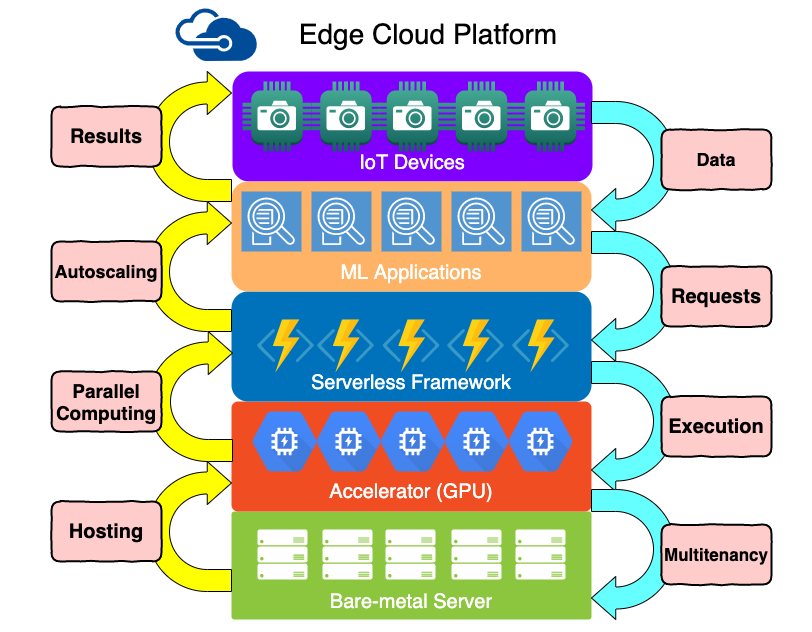
\includegraphics[scale=0.3]{figures/edge_platform}
    \caption{The abstract design of an edge cloud platform leveraging serverless framework and GPUs for executing distributed machine learning applications in IoT settings.
\label{fig:edge}}
\end{figure}

As depicted in Figure~\ref{fig:edge}, we envision an ideal edge cloud platform, to which IoT devices transmit data in batches for training and inference applications. The hierarchy of the platform has five layers: (1) \textbf{bare-metal server} cluster hosts hardware using multitenancy; (2) \textbf{accelerators} (i.e. GPUs) provide computational power by parallel computing; (3) \textbf{serverless framework} autoscales function execution upon the rate of requests; (4) \textbf{machine learning application} receives streaming data from (5) \textbf{IoT devices} and returns results (i.e. classification, regression, etc.)

In this paper, we present STOIC (Serverless TeleOperable Hybrid Cloud) that embraces such designing philosophy. Unique to STOIC, however, is its offloading system which intelligently places the application workload on edge and cloud systems based on its precise prediction of total latency. We consider three major contributions from this work: (1) we design and implement a serverless framework serving IoT requests by leveraging GPU acceleration. (2) we investigate feedback control mechanism and various analytical methodologies to precisely model the unstable edge and public cloud environments. (3) we test the efficacy of using this extended serverless model for machine learning applications that span edge-cloud systems, and empirically evaluate the performance of doing so. Using real workloads and deployments, we find that STOIC reduces the total response time of the benchmark application by 55\% (2.3x speedup), compared with baseline scenario. In the evaluation of duplicator mode, STOIC promptly responds to 95\% (2 GPUs) - 97\% (1 GPU) of requested workloads with the least latency in a 24-hour experiment. 
\fi



\section{STOIC}
\label{sec:stoic}
\begin{figure}
    \centering
    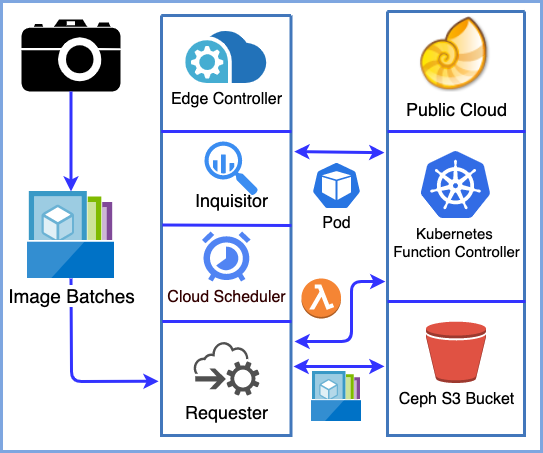
\includegraphics[scale=0.5]{figures/STOIC.png}
    \caption{The STOIC Architecture \label{fig:STOIC}}
\end{figure}


To leverage hardware acceleration and distributed (multi-cloud) scheduling within a serverless architecture, we have developed STOIC, a framework for distributing and executing analytics applications across multi-tier IoT (sensing-edge-cloud) settings. Specifically, STO\-IC optimizes the end-to-end process of packaging, transferring, scheduling, executing, and result retrieval for machine learning applications in these settings.  

Figure~\ref{fig:STOIC} shows the distributed components of STOIC. At the edge, STOIC gathers application input data, determines whether the lower application latency will be achieved by processing the data on the edge or in the cloud, and then actuates the application's computation (with the necessary data) using the ``best'' choice. The public cloud component manages whatever cloud resources are needed to receive the data from the edge, trigger the computation, and return the results to the edge.  The edge and cloud systems mirror each other, running Kubernetes~\cite{ref:k8s-web,ref:k8s} overlaid with kubeless~\cite{ref:kubeless}, to provide a uniform infrastructure for the framework.

Our system design is motivated by a need to classify wildlife images in a location where it is possible to site a relatively powerful edge system but where network connectivity is poor.  In this paper, we report on the use of STOIC  for processing images from multiple, motion-triggered camera traps (sensors) deployed to a wildlife reserve currently used to study ecological land use.
%monitor wildlife across the Sedgwick Natural Reserve~\cite{ref:sedgwick}.

\subsection{Edge Controller} 

The STOIC edge controller is a server that runs in an
out-building at the reserve. It communicates wirelessly with the sensors and triggers analysis and computation upon their arrival. The edge controller is connected to a research facility (which has full Internet connectivity) 
%remove for blind: the UCSB campus
via a microwave link. When a camera trap detects motion, it takes photos and persists the images in flash storage buffer, where human experts would label images for training tasks. Periodically, sensors transfer saved photos to the edge controller. During a transfer cycle, the edge controller compresses and packages all images generated and transfers the package to the public cloud, if/when necessary. STOIC runs on the edge controller and its executions are triggered by the arrival of image batches. 

As an intermediate computational tier between the sensors and the public cloud, the edge controller can be placed anywhere, preferably near the edge devices, to lower the response latency for the data processing and analytics applications. It consists of three major components: 
\begin{itemize}
\item The \textbf{cloud scheduler} predicts the total latency based on historical measurements for each available runtime. 
\item The \textbf{requester} takes as input the runtime and cloud predicted by the scheduler to have the least latency.  The requester stores the image package in an object storage service running in this cloud. It then triggers a serverless function (running in a Kubernetes pod) via a RESTful HTTP request to process the images.
%public cloud. If the public cloud is chosen, the requester
%first transfers the image batch to a dedicated Ceph~\cite{ref:ceph} 
%S3 bucket in the public cloud. 
\item The \textbf{inquisitor} monitors public cloud deployment time. To enable this, it periodically in the background deploys each runtime (using Kubernetes pods~\cite{ref:pods}) and records the deployment times in a database. No task/process is executed in this process (the runtime is simply deployed and taken down). We use the inquisitor to establish the historical time series for predicting the deployment latency of remote runtimes.
\end{itemize}

The edge cloud that we use in this study is deployed at a research reserve and is connected via the Internet.  It consists of a cluster of three Intel NUCs~\cite{ref:nucs} (6i7KYK), each with two Intel Core i7-6770HQ 4-core processors (6M Cache, 2.60 GHz) and 32GB of DDR4-2133+ RAM connected via two channels. The cluster is managed using the Eucalyptus cloud system~\cite{ref:euca}, which mirrors the Amazon Web Services (AWS) interfaces for Elastic Compute Cloud (EC2) to host Linux virtual machine (VM) instances and Simple Storage Service (S3) to provide object storage. The STOIC edge runtime uses Kubernetes and kubeless for serverless function execution and S3 (i.e. walrus) for object storage on the edge cloud.
 
\subsection{Public/Private Cloud}

To investigate the use of the serverless architecture with hardware acceleration, we employ a shared, multi-university, GPU cloud, called Nautilus~\cite{ref:nautilus}, as our remote cloud system. Nautilus is an Internet-connected, HyperCluster research platform developed by researchers at UC San Diego, the National Science Foundation, the Department of Energy, and multiple, participating universities globally.  Nautilus is designed for running data and computationally intensive applications. It uses Kubernetes~\cite{ref:k8s} to manage and scale containerized applications. It also uses Rook~\cite{ref:rook} to integrate Ceph~\cite{ref:ceph} for object storage. As of May 2020, Nautilus consists of 176 computing nodes across the US and a total of 543 GPUs in the cluster. All nodes are connected via a multi-campus network. In this study, we consider Nautilus a public cloud that enables us to leverage hardware acceleration (GPUs) in the serverless architecture. The STOIC cloud/GPU runtimes use Kubernetes and kubeless for serverless function execution and Ceph for object storage on the public cloud.

A major challenge that we face with such deployments is hardware heterogeneity and performance variability. On Nautilus, we have observed 44 different types of CPU (e.g. Intel Xeon, AMD EPYC, among others) and 9 GPU types (e.g. Nvidia 1080Ti, K40, etc.). Both CPUs and GPUs of different types have different performance characteristics. Moreover, the object storage service is run on dedicated nodes that are distributed globally.

This heterogeneity impacts application execution time (which STOIC attempts to predict) in three significant ways. First, different CPU clock rates affect the transfer of datasets from the main memory to GPU memory. Second, there is significant latency and performance variability between runtimes and the storage service (which hold the datasets and models). Third, the multi-tenancy of nodes (common in public cloud settings) allows other jobs to share computational resources with our applications of interest at runtime. 

These three factors negatively make it difficult for users to determine which runtime to use (to reduce application turn-around time) and when to execute locally (avoiding public  cloud use altogether). With STOIC, we address these challenges via a novel scheduling system that adapts to this variability. In our results, we ensure reproducibility (avoiding network performance variability) by confining nodes and GPUs (still heterogeneous) to a single Nautilus region.

\subsection{Runtime Scenarios}

To schedule machine learning tasks across hybrid cloud deployments, we define four runtime scenarios: \textbf{(A)} \textit{Edge} - A VM instance on the edge cloud with AVX2~\cite{ref:avx} support; \textbf{(B)} \textit{CPU} - A Kubernetes pod on Nautilus containing a single CPU with AVX2 support~\cite{ref:avx}; \textbf{(C)} \textit{GPU1} - A Kubernetes pod on Nautilus containing a single GPU; \textbf{(D)} \textit{GPU2} - A Kubernetes pod on Nautilus containing two GPUs.  STOIC considers each of these deployment options as part of its scheduling decisions. Users can parameterize STOIC with their choice of deployment or allow STOIC to automatically schedule their applications.

\subsection{Execution Time Estimation}

As depicted in Figure~\ref{fig:STOIC}, the STOIC's edge controller listens for image batches from the remote camera traps and makes machine learning job requests. After a preset period (parameterizable but currently set to an hour), STOIC estimates total response time~($T_s$) of a requested batch, based on 4 different runtime scenarios. The total response time ($T_s$) includes data transfer time~($T_t$), runtime deployment time~($T_d$), and the corresponding processing time~($T_p$). We define total response time~($T_s$) as $T_s = T_t + T_d + T_p$.
 
\subsubsection{Transfer time ($T_t$)} 

$T_t$ measures the time spent in transmitting a compressed batch of images from the edge controller to edge cloud and public cloud. We calculate transfer time as ${T_t = F_b / B_c}$ where $F_b$ represents the file size of batch and $B_c$ represents the bandwidth at the moment provided by a bandwidth monitor at the edge controller. 
 
\subsubsection{Runtime deployment time ($T_d$)} 

$T_d$ measures the time Nautilus uses to deploy requested kubeless function. Since the scarcity of computation, it is common that multi-GPU runtime takes longer to deploy than single-GPU and CPU runtimes. Note that, for \textit{edge} runtime, the deployment time zeroes out since STOIC executes the task locally in the edge cloud.
 
\begin{figure*}
    \centering
    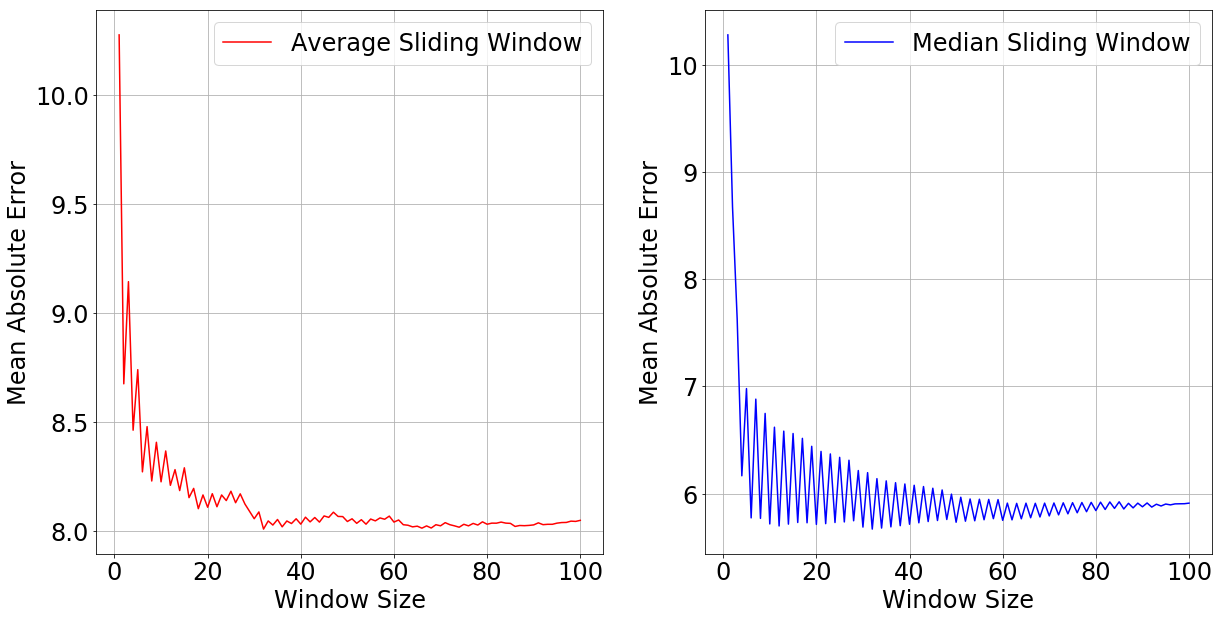
\includegraphics[scale=0.31]{figures/deployment}
    \caption{The Mean Absolute Error (MAE) of deployment time for the GPU1 runtime. The x-axis is the window (history) size. The left subplot is MAE when STOIC uses the average sliding window, the right subplot is MAE when STOIC uses the median sliding window.
\label{fig:deployment}}
\end{figure*}

 
\begin{table}
\centering
\resizebox{320pt}{!}{
\scriptsize
\resizebox{\columnwidth}{!}{
\begin{tabular}{|c|c|c|c|} 
\hline
& & \textbf{Optimal} & \textbf{Minimum}  \\
\textbf{Modeling} & \textbf{Runtime} & \textbf{Window Size} & \textbf{MAE}  \\
\hline
AutoReg & CPU & 15 & 8.977 \\
\hline
AutoReg & GPU1 & 15 & 9.605 \\
\hline
AutoReg & GPU2 & 15 & 17.918 \\
\Xhline{2\arrayrulewidth}
Avg. SW & CPU & 33 & 7.714 \\
\hline
Avg. SW & GPU1 & 31 & 8.006 \\
\hline
Avg. SW & GPU2 & 91 & 16.52 \\
\Xhline{2\arrayrulewidth}
Med. SW & CPU & 13 & \textbf{5.96} \\
\hline
Med. SW & GPU1 & 31 & \textbf{5.668} \\
\hline
Med. SW & GPU2 & 27 & \textbf{14.48} \\
\hline
\end{tabular}
}
}
\caption{Mean Absolute Error of three time series modeling methods for runtime deployment time: auto-regression (AutoReg), average sliding window (Avg. SW), and median sliding window (Med. SW). The median sliding window achieves the lowest minimum MAE at optimal window size (that with the lease MAE) for all three runtimes. \label{tab:deployment}}

\end{table}
 

Because Nautilus is a shared cloud system, we observe significant variation in deployment time on Nautilus for different times of the day. To accurately predict deployment time, we analyze deployment times as a time series using three methods: (1) auto-regression modeling, (2) average sliding window, and (3) median sliding window. Auto-regression~\cite{ref:autoreg} is a time series modeling technique based on the auto-correlation between previous time steps and the following ones. The average sliding window is the moving average~\cite{ref:moveavg} scanning through the time series by a fixed-length window. Similarly, the median sliding window captures the moving median cross the time series. All window sizes used for three modeling processes are optimized based on historical data of deployment time~($T_d$) in January 2020. We then compare the minimum Mean Absolute Error (MAE) from each to select the best modeling methodology. 

In this example, we consider a time series of 1244 data points for each runtime. Figure~\ref{fig:deployment} shows representative analytics for GPU1 deployment time, in which MAE oscillates as window size varies. We observe that the median sliding window reaches a lower minimum MAE than the average sliding window at optimal window size. As listed in Table~\ref{tab:deployment}, all three runtimes achieve the lowest minimum MAE using the median sliding window. Therefore, STOIC adopts this methodology for deployment time prediction. 

The inquisitor measures and records deployment time for each public cloud runtime every minute (called the inquisitor period). After the inquisitor records 10 new measurements (called the calibration period), the scheduler recomputes the window size over the previous 100 measurements that result in the minimum MAE. It then uses this minimum MAE window size to estimate of deployment time when jobs arrive. The inquisitor period, calibration period, and maximum window size are all modifiable.
%explain here how STOIC uses this data to adapt window size and when the estimate
%is computed.  Is this estimate what is used by the scheduler?
%%STOIC slides this window as new deployment measurements are logged by the
%%inquisitor.  The default window size in our experiments is 100 
%%measurements; STOIC calculates a
%%new estimate every 10 measurements. Both of these parameters are modifiable.

%The number of data points
%used in the analysis (i.e. 100 by default) and the interval of calibration (i.e.
%every 10 executions by default) are both parameterizable, to allow for
%tuning and trading off performance and accuracy. By default (used in our 
%results), the inquistor
%measures deployment time of the public cloud runtimes every minute.
%CJK
 
\subsubsection{Processing time~($T_p$)} 

$T_p$ is the execution time of a specific machine learning task and the target of task scheduling across the hybrid cloud. STOIC formulates a linear regression on execution time histories of STOIC jobs, and uses it to predict processing time relative to input (image batch) size. Specifically, we use Bayesian Ridge Regression~\cite{ref:brr} due to its robustness to ill-posed problems (relative to ordinary least squares regression~\cite{ref:ols}). STOIC queries the database for the most recent processing time data (e.g. 10 data points) for each regression. This ensures that the parameters of the regression line reflect the current runtime performance.

\begin{algorithm}[]
\caption{Random Sample Consensus}
\label{algo:ransac}
\SetAlgoLined
\KwData{
(1) Observation set of Process time $T_p$\\
(2) Bayesian Ridge Regression model $M$\\
(3) Minimum sample size $n$\\
(4) Residual threshold $t$\\
(5) Maximum iteration $k$ \\
(6) Required inlier size $d$ \\ 
(7) Minimum Root Mean Square Error $e$ \\
}
\KwResult{A set of parameters that best fits the data}
 \While{iterations $\leq$ k}{
    curr\_sample := $n$ data points from observation\;
    curr\_model := $M$ regressed on curr\_sample\;
    fit\_data := empty set\;
    \For{ every data point $p$ in curr\_sample}{
        \uIf{error of $p$ $\leq$ $t$}{
            $p$ $\to$ fit\_data\;
        }
    }
    \eIf{fit\_data size $\geq$ $d$}{
        curr\_error := average error in fit\_data\;
        \uIf{curr\_error < $e$}{
            Update $M$ and $e$
        }
    }{Increment iteration}
 }
 return $M$
\end{algorithm}
 
As part of our investigations into this approach, we have found that this approach is highly susceptible to outliers. The root cause of these outliers is sporadic congestion and maintenance (for nodes, networking, etc.) of the public cloud. Deviating significantly from the average, outliers skew the regression line and overestimate the runtime latency for extended periods (due to the windowing approach). We thus augment regression using a random sample consensus (RANSAC) technique~\cite{ref:ransac}, which iteratively removes outliers from the regression. The algorithm~\ref{algo:ransac} illustrates our RANSAC approach in STOIC.

 
 \begin{figure*}
    \centering
    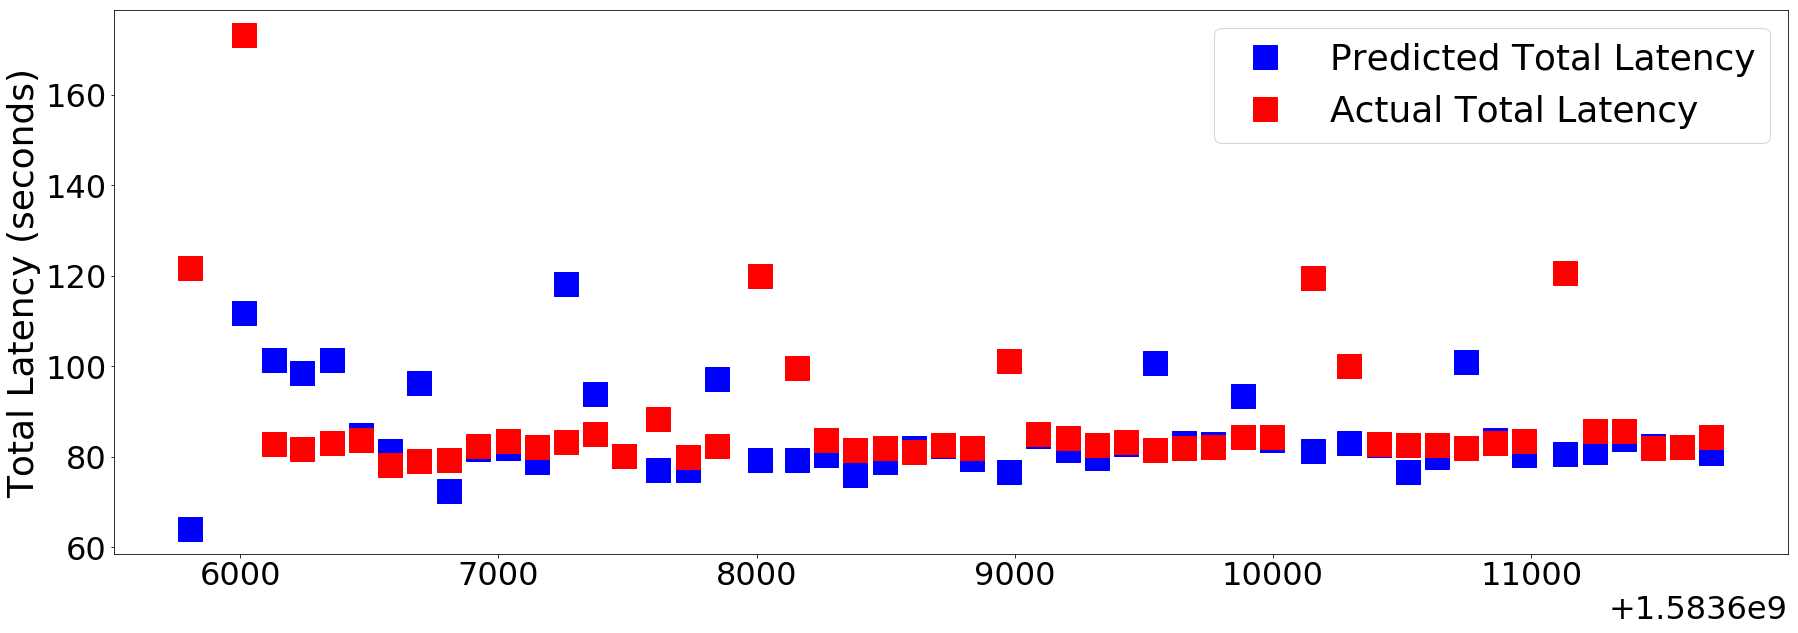
\includegraphics[scale=0.20]{figures/timeline.png}
    \caption{The comparison of predicted and actual total latency on 50 GPU1 benchmark executions with 150-image batch size. The x-axis is the epoch time and the y-axis is the total latency. \label{fig:timeline}}
\end{figure*}
 
 \subsubsection{Adaptability}
 
To verify that STOIC's estimation of execution time captures the actual latency of the public cloud, we execute the application 50 times with 150-image batch using the GPU1 runtime. Depicted in Figure~\ref{fig:timeline}, we observe that actual total latency varies significantly and predicted total latency has a non-negligible difference from the actual total latency at the beginning of the experiment. However, over time, as STOIC learns the various latencies of the system, the difference is significantly reduced. In Table~\ref{tab:timeline}, we report the percentage mean absolute error (PMAE), which we compute as the MAE divided by mean latency. The decrease in all three PMAE values in the second half of the execution trace also show STOIC's adaptability.

\begin{table}
\centering
\resizebox{340pt}{!}{
\scriptsize
\resizebox{\columnwidth}{!}{
\begin{tabular}{|c|c|c|c|} 
\hline
 & \textbf{Deployment $T_d$} & \textbf{Processing $T_p$} & \textbf{Total $T_s$}  \\
\hline
First Half & 42.7\% & 11.2\% & 15.8\% \\
\hline
Second Half & 29.2\% & 5.3\% & 9.2\% \\
\hline
\end{tabular}
}

}
\caption{The percentage mean absolute error (PMAE) of deployment, processing, and total latency. PMAE is a latency-normalized metric and calculated as MAE divided by mean latency, which indicates the residual in a measured period. The decline of three latency metrics in the second half demonstrates the adaptability of STOIC.
\label{tab:timeline}}
\end{table}

\begin{figure*}
\centering
\begin{minipage}{.45\textwidth}
  \centering
  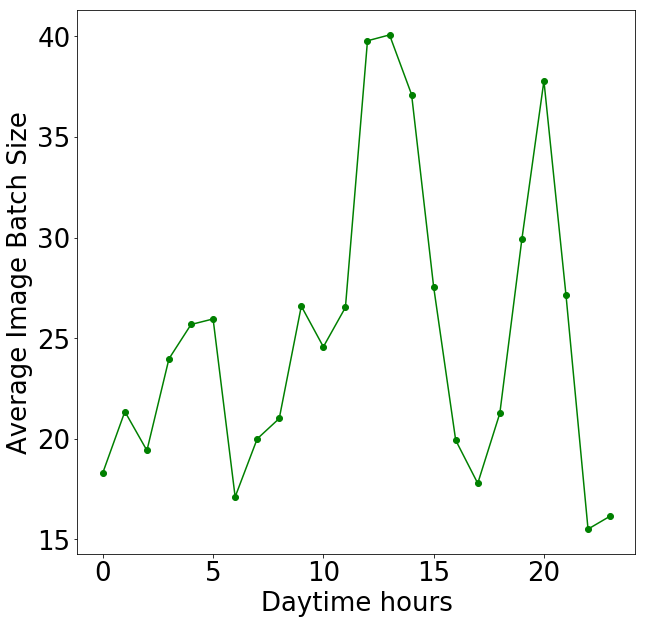
\includegraphics[width=\linewidth]{figures/Hourly_act.png}
\end{minipage}%
\hspace{0.5in}
\begin{minipage}{.45\textwidth}
  \centering
  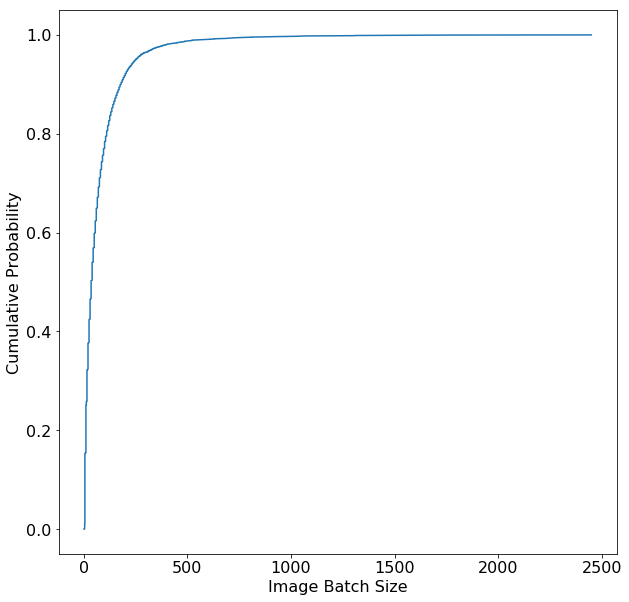
\includegraphics[width=\linewidth]{figures/ecdf.png}
\end{minipage}
\caption{Wildlife Hourly Activity Level (left graph) and its Conditional Empirical Cumulative Distribution Function (right graph). The left graph demonstrates the mean activity level of wildlife throughout the daytime. Based on the curve, 1 PM and 8 PM are two peak hours of animal activities.  The right graph shows the empirical CDF, which STOIC randomly samples for image batches to drive our faster-than-real time empirical evaluation of the system.\label{fig:hour_act_and_cdf}}
\end{figure*}

\ignore{
\begin{figure*}[t] \centering 
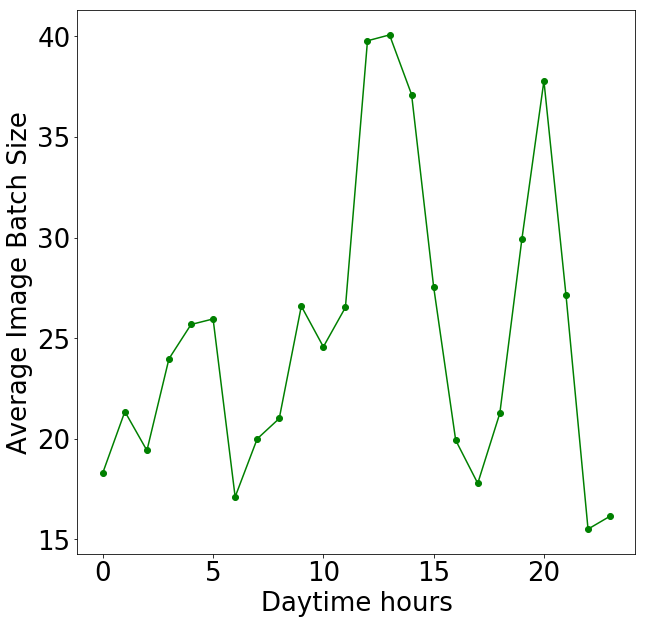
\includegraphics[scale=0.4]{figures/Hourly_act.png}
\caption{Wildlife Hourly Activity Level. The figure demonstrates the mean activity level of wildlife throughout a day. Based on the curve, 1PM and 8PM are two peak hours of animal activities.
\label{fig:hour_act}}
\end{figure*} 
 
 
\begin{figure*}[t] \centering 
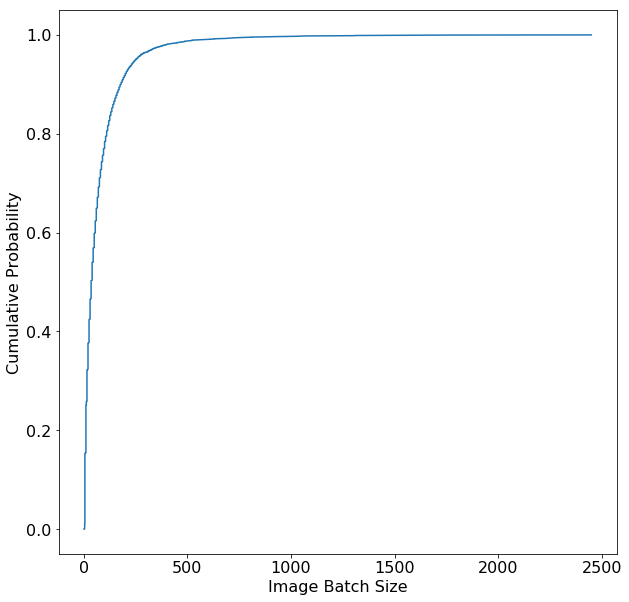
\includegraphics[scale=0.4]{figures/ecdf.png}
\caption{Conditional Empirical Cumulative Distribution Function. The STOIC image batch simulator is based on this function and random probabilities [0, 1) from a uniform distribution.
\label{fig:cecdf}}
\end{figure*} 
}
 
\subsection{Workload Generation}
\label{sec:workloadgen}

To drive our empirical evaluation in faster-than-real time,  we construct a workload generator from image batch histories (traces) collected by our camera traps. We consider the set of images that occur together within an hour (i.e. due to motion events) a batch. Our camera trap trace, starting on July 13th, 2013 and ending Jan. 15th, 2017, comes from a fixed camera located at a watering hole in a remote area of our research reserve. The trace contains images of bear, deer, coyote, puma, and birds as well as wind-triggered empty images and other animals.

After excluding camera maintenance periods (gaps), we  extract 1136 effective days (27264 hours) of data. The maximum size of hourly image batch is 2450, whereas the minimum size is unsurprisingly zero, which constitutes 18139 hours out of 27264 hours (66.53\%). On average, an hourly image batch size contains 25 images. The left graph in Figure~\ref{fig:hour_act_and_cdf} illustrates the wildlife  hourly activity level based on the image batch size. We infer from the curve that 1 PM and 8 PM are two peak hours of animal activity.

Specifically, we construct a conditional empirical cumulative distribution function (ECDF) based on the probability definition of  $Pr(x < K | x > 0)$, where x is the image batch size and K is the cutoff value. This conditional ECDF effectively represents the trajectory of the animal activity level and makes the evaluation empirical. The right graph in Figure~\ref{fig:hour_act_and_cdf} plots the conditional ECDF. 
The x-axis is the image batch size ranging from zero to 2450, whereas the y-axis is the cumulative probability. The STOIC workload generator draws image batch sizes by
randomly sampling this ECDF.
%The sampling procedure is as follows.  During the execution of STOIC, 
%the simulator first generates a
%random number in [0, 1) from a uniform distribution and secondly retrieves the
%corresponding image batch size from the conditional ECDF. 
Using this process, we are able to evaluate and conclude by replaying the image stream from the camera traps in fast-than-real time for the purposes of comparative evaluation.

%, regarding STOIC's
%performance and efficiency by a real-world streaming data flow.



 \subsection{Implementation}

%Considering performance and interface, 
We implement STOIC using Golang~\cite{ref:golang}. Golang provides high-performance execution (vs scripting languages) and a user-friendly interface~\cite{ref:client-go} to Kubernetes and database technologies. STOIC currently supports machine learning applications developed using the TensorFlow framework~\cite{ref:tensorflow} and can be easily extended to permit other machine learning libraries.
%by extending the runtime
%environment.
 
As mentioned previously, the STOIC serverless architecture leverages kubeless~\cite{ref:kubeless}. As a Kubernetes-native serverless framework, kubeless uses the Custom Resource Definition (CRD)~\cite{ref:crd} to dynamically create functions as Kubernetes custom resources and launches runtimes on-demand. For specific machine learning tasks that STOIC executes, we build custom Docker images that we upload to Docker Hub~\cite{ref:dockerhub} in advance. When the function controller receives a task request, it pulls the latest image from Docker Hub before launching the function. This deployment pipeline makes the runtime flexible and extensible for evolving applications. 
%To create a consistent serverless environment, we install and configure
%minikube~\cite{ref:minikube} and kubeless~\cite{ref:kubeless} on the edge
%cloud. They enable the edge cloud to execute and respond to serverless
%function requests in the same manner as Nautilus. To further reduce the
%deployment time on the minikube cluster, 

To leverage the computational power of our CPU systems, we compile Tensorflow with AVX2, SSE4.2 \cite{ref:avx}, and FMA~\cite{ref:fma} instruction set support. We use this optimized version of Tensorflow on both the edge and public clouds.
%From our previous test result
%in~\cite{ref:stoic}, we observe significant speed-up from the customized
%library on CPU runtime. Therefore, we use this Tensorflow configuration on
%both the edge cloud and Nautilus.
 
To enable GPU access by serverless functions (available in the public cloud), we equip our Docker container with NVIDIA Container Toolkit~\cite{ref:nvidia}. This includes the NVIDIA runtime library and utilities, which link serverless functions to NVIDIA GPUs. We also install CUDA 10.0 and cuDNN 7.0 to support the machine learning libraries.
 
 
 \subsection{Workflow}

\begin{figure}[t] \centering 
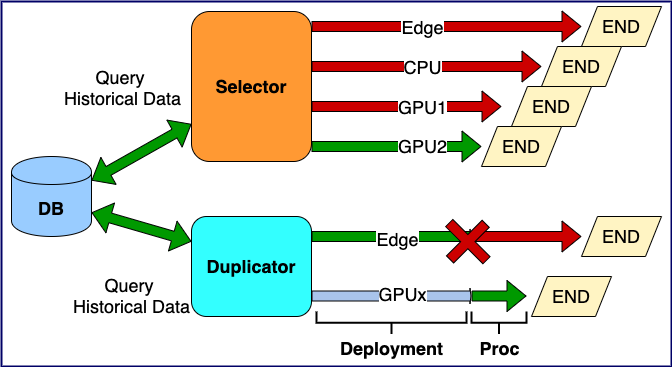
\includegraphics[scale=0.5]{figures/selector_duplicator.png}
\caption{The selector and duplicator modes of STOIC. 
\label{fig:duplicator}}
\end{figure}


STOIC considers two workflows upon receiving an image batch: 
selector mode and duplicator mode. Both are depicted in Figure~\ref{fig:duplicator}. In selector mode, STOIC predicts the total response times~($T_s$) of the four deployment options: Edge, CPU, GPU1, and GPU2.  It then selects the runtime with the shortest estimated response time and deploys it locally (Edge) or remotely (non-Edge). Once deployed, the pod notifies the STOIC requester at the edge which then triggers the serverless function via an HTTP request. When the task completes, the pod notifies the requester, which retrieves the results and runtime metrics from the deployment and stores them in the database for use by the scheduler.

To handle deployment failure, STOIC implements a retry mechanism using exponential back-off. Starting at 100 milliseconds, STOIC waits 2X length of time for retrying the deployment on Nautilus. After 10 failed attempts, STOIC claims timeout and returns an error.

STOIC also attempts to reduce startup time (i.e. cold starts) at both the edge and public cloud. On the edge cloud, STOIC creates a standby pod to serve the incoming request upon application invocation. On the public cloud, STOIC triggers a function with a single image to retrieve and cache the base model in memory at each pod.
 
%Once Nautilus successfully deploys the serverless function, it informs the
%edge cloud's requester to trigger the function via an HTTP request. To cope
%with the cold starts~\cite{ref:coldstart}, STOIC triggers the function with
%the least amount of input data to ensure the function caches the model in
%memory. When the task completes, the requester retrieves the results and
%runtime metrics, and transmits them back to the edge controller. Finally, the
%edge cloud logs the results and metrics to the database for use in later
%predictions. 

We observe from Table~\ref{tab:timeline} that there are significant variations in the deployment time of the runtimes on the shared public cloud. To enable STOIC to adapt to this variability, we consider a second workflow called \textbf{duplicator} mode. Using this mode, when the scheduler selects a public cloud runtime (i.e. CPU, GPU1, GPU2), the requester \textit{also} deploys the job on the edge cloud. It then terminates edge cloud execution if the remaining time at edge cloud is longer than the expected processing time ($T_p$) at the GPU runtime once deployment completes. This ``lagging decision'' mechanism reduces the variability of deployment time in the prediction. As a result, STOIC must only consider processing time, which is more accurately predicted, to deploy tasks. Note that duplicator mode is less energy-efficient because it runs tasks regardless of latency prediction and may waste cloud resources by killing the function in the middle. However, if such waste can be tolerated, significant prediction accuracy and latency reduction are possible.

In addition, the inquisitor running in the background deploys the public cloud runtimes periodically and stores the deployment time duration in the database for use in the prediction. We set a timeout (i.e. 10 minutes) to terminate this process for any unresponsive deployment. That is, the inquisitor marks the runtime unavailable (from the point of view of the requester) when the deployment hits the set timeout. The inquisitor continues to attempt deployment of this runtime periodically and makes it available to the requester once a deployment attempt is successful.

To bootstrap the system, STOIC executes two representative tasks for an application for each runtime in both the edge and public cloud. It uses these data points as a basis for its processing time estimation by linear regression. STOIC performs this bootstrapping each time a new version of the application is uploaded by the developer.

%Extended from the initial version, we enable STOIC to take application name
%and versioning information as input. Once a new application is deployed or the
%existing application is updated, the regression initiator automatically
%executes two tasks based on the current application and version for each
%runtime scenario. These two data points 
%initialize the incoming regressions
%and predictions across the edge and public cloud.

%. Seen in Figure~\ref{fig:duplicator}, the
%edge cloud then schedules only one request, using the payload of
%compressed image batch and runtime information. Upon execution, the edge cloud
%triggers the serverless function locally if/when the choice is the \textit{edge}
%runtime. %Edge deployment is typically selected when batch size is small. 

%For large batch sizes, STOIC typically schedules one of the three public
%runtime options. For these three scenarios, the edge cloud first requests the
%deployment on the public cloud. It then sends the payload to public cloud
%storage. The public cloud then deploys the runtime on nodes that satisfy the
%node affinity configuration. 



\section{Evaluation}
\label{sec:results}
In this section, we empirically evaluate STOIC's performance on image processing tasks. We implement the application as a serverless function for STOIC to schedule and execute.

In each experiment, STOIC determines which resource to use for function execution (among a small set of feasible choices). We then run the function on \textit{all} resources and compare the choice made by STOIC to the best (shortest duration) execution across all possible choices.

\subsection{Experimental Setup}

The image processing application that we use as a benchmark classifies animal images from a wildlife monitoring system.
%called ``Where's The Bear"
%(WTB)~\cite{ref:wtb}. ``Where's The Bear" is an end-to-end distributed data
%acquisition and analytics system that automatically analyzes camera trap
%images collected by cameras sited at the Sedgwick Natural
%Reserve~\cite{ref:sedgwick} in Santa Barbara County, California. The WTB
Our deployment includes an edge cloud located near the cameras where it acquires the image data. The edge cloud is connected via a slow (microwave) link to a private cloud located at a research facility located approximately 50 miles from the site. In this work, we explore using the Nautilus distributed GPU cloud~\cite{ref:nautilus} as the public cloud, in conjunction with the edge cloud to optimize image classification on a convolutional neural network (CNN)~\cite{ref:cnn} implemented by Tensorflow and Scikit-learn~\cite{ref:scikit}. 

In total, there are five classes that we consider: Bird, Fox, Rodent, Human, and Empty, by which we label images for training tasks and evaluate model by inference. Since class size is unbalanced due to the frequency of animal occurrences, we up-sample minority classes (e.g. fox) using the Keras ImageDataGenerator~\cite{ref:keras}. Doing so ensures that the classification model is not biased. We resize every image in the image dataset to $1920 \times 1080$, and for each class, the dataset contains 251 images used to train the CNN model. Once model training is complete, the application stores this model in hdf5 format in object storage at both edge cloud and Nautilus.

As described previously, STOIC moves images from the wildlife refuge to the public cloud in batches. To better harness the multiple GPU runtime of the public cloud, the application spawns a process (wor\-ker) for each GPU and adds all images in a batch to a shared asynchronous queue. Upon the execution, workers remove images (one at a time) from the shared queue until it is exhausted. This mechanism ensures multiple GPU runtimes evenly divide the workloads among GPUs and achieve quasi-linear acceleration at the application level, where the perfect linear speed-up is unattainable because of model loading and memory transfer overhead~\cite{ref:multi_gpu}. 


\iffalse
\subsection{Deployment Options}

We explore four different deployment options on STOIC: 
\begin{itemize}
\item a node of the edge cloud (Edge), 
\item on the controlling CPU (an x86 processor) that Nautilus uses to move
data in and out of one or more GPUs (CPU),
\item on one GPU in Nautilus (GPU1),
\item on two GPUs in Nautilus (GPU2).
\end{itemize}
On the edge cloud, the application begins immediately when a camera delivers an image batch.  To use Nautilus, however, the image batch must first traverse the network from the edge cloud to Nautilus (thereby incurring an additional transfer time) and then Nautilus must schedule a ``pod'' (containing either one or two GPU in this study) before the Nautilus CPU or any GPU can begin running.  We define the time that Nautilus requires for pod scheduling as ``deployment time.''~\footnote{Note that Nautilus currently allows non-priviledged users to request up to 8 GPUs, but the deployment times for requests of greater than 2 are usually large as to make them superfluous. That is, a GPU request for more than two GPUs is rarely, if ever successfully, satisfied in the shortest possible time.} Finally, the run time is the time required by a resource (Edge, CPU, GPU1, and GPU2) to complete the CNN training.  

We do not explore the possibility of overlapping transfer time, deployment time, and run time and we do not model the time required to return the trained model to the edge cloud. Thus the total response time is the sum of the transfer time, the deployment time, and the run time for an image batch. On the edge, the transfer times and deployment times are zero.
\fi



\begin{figure*}[t] \centering 
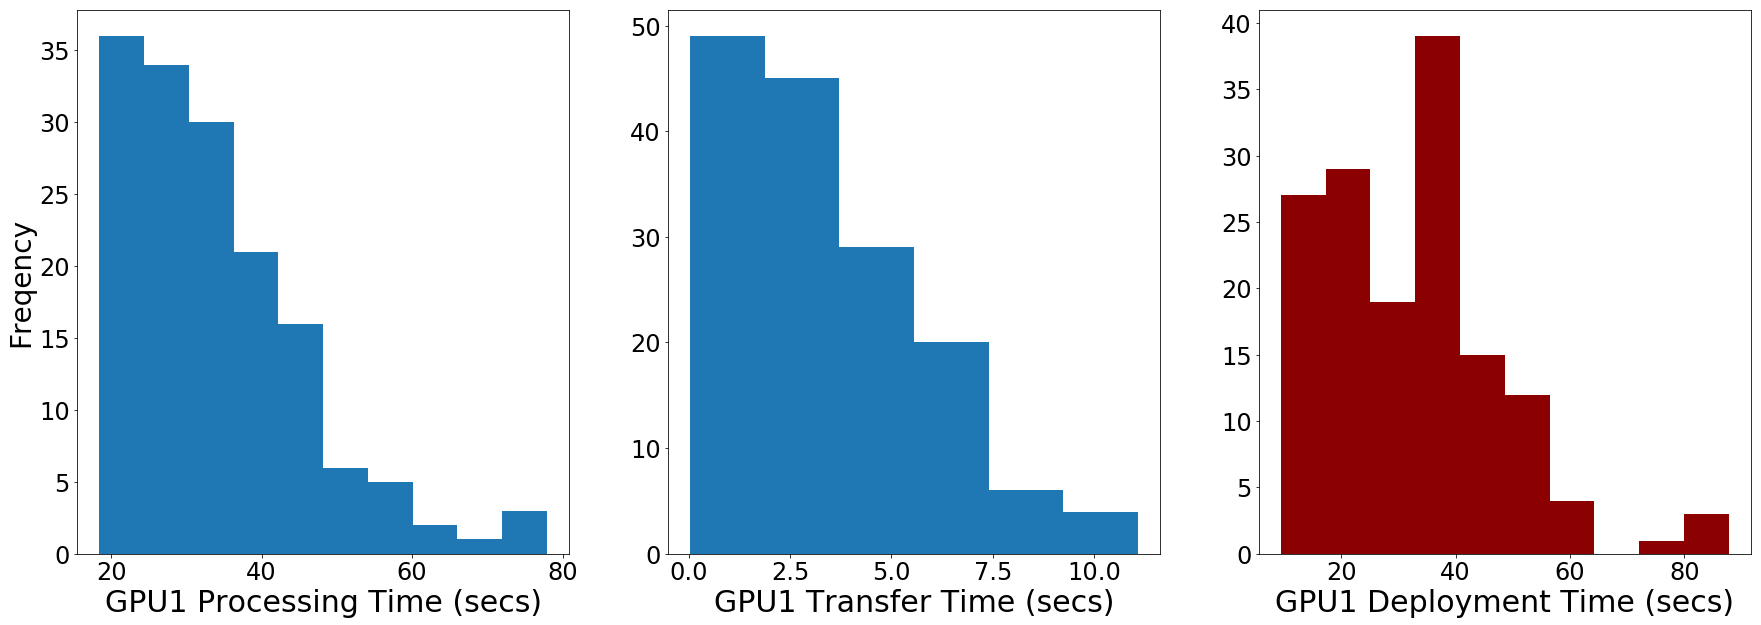
\includegraphics[scale=0.22]{figures/gpu1_latency.png}
\caption{The distribution of three components in total response time~($T_s$) of 150 executions on GPU1 runtime: Processing time ($T_p$), Deployment time ($T_d$), and Transfer time ($T_t$). The x-axis represents the time range, while the y-axis is the frequency of executions. The deployment time, which is depicted in the red histogram, is volatile and error-prone to prediction.
\label{fig:breakdown}}
\end{figure*}

To drive this experiment, we use the workload generator described in Section~\ref{sec:workloadgen} to facilitate faster-than-real time evaluation of STOIC. The generator uses an image series and their inter-arrival patterns from a camera trap image corpus ranging from 2013 to 2017. Figure~\ref{fig:breakdown} shows example histograms for processing time, transfer time, and deployment time on Nautilus for GPU1 runtime using 150 batches drawn from the workload generator. On the x-axis, we show the elapsed time for processing time, transfer time, and deployment time respectively. Note that processing time and transfer time are relatively stable compared to deployment time. 

\subsection{Selector Evaluation}

We first evaluate STOIC selector mode for a 24-hour period consisting of 162 image batches, the sizes of which are drawn randomly from the workload generator. Each batch is executed on the edge cloud, on the Nautilus CPU, on one Nautilus GPU, and two Nautilus GPUs. Over the test period, the STOIC Selector chooses the fastest (lowest total response time) from among these four options $149$ times out of the $162$ runs or $92\%$ of the time. That is, STOIC correctly identifies the fastest option with a success rate of $92\%$.

Further, the optimal selection (i.e. an oracle selection that is $100\%$ correct) would have resulted in an aggregate total latency of $10022$ seconds, whereas the worst case has aggregate latency $35940$ seconds compared to a STOIC aggregate latency of $10770$ seconds.  Thus STOIC achieves an aggregate latency that is $7.4\%$ slower than optimal, but $70\%$ ($3.33$x) faster than the worst case.

%Table~\ref{tab:selector} summarizes these results. In the
%table, we report the success rate, the percentage of optimal, and the
%percentage of worst case aggregate response times achieved by STOIC. 

%\begin{table}[t] 
%\begin{centering}
%\captionsetup{justification=centering}
%\scriptsize
\resizebox{\columnwidth}{!}{
\begin{tabular}{|c|c|c|} 
\hline
\textbf{Success Rate} & \textbf{versus Optimal} & \textbf{versus Worst Case}\\
\hline
$92\%$ & $105\%$ & $30\%$ \\
\hline
\end{tabular}
}

%\end{centering}
%\caption{
%STOIC Selector results. The success rate is the percentage of correct decisions
%(out of 162 trials) made by STOIC.  ``Optimal'' shows the percentage of the
%optimal selection aggregate response time and ``Worst Case'' shows the percentage of the worst case 
%selection aggregate response time made by STOIC.}
%\label{tab:selector}
%\end{table}

We further analyze the data points where STOIC made erroneous selections and found two sources of error. First, the most error occurs around two batch sizes where the total response times of runtime have approximately the same latency. To be specific, the edge and GPU runtimes cross over at 35 image batch size and 90 image batch size for the GPU1 and GPU2 runtimes. At these cross-points, the close predictions of latency lead to incorrect selection.~\cite{ref:stoic2020} Second, the deployment times for GPU runtime are volatile and error-prone to prediction. As a representative instance, Figure~\ref{fig:breakdown} demonstrates the distribution of processing time ($T_p$), transfer time ($T_t$) and deployment time ($T_d$) of GPU1 runtime. We observe geometric distribution from the histogram of processing time and transfer time, whereas deployment time varies irregularly with many outliers. These two phenomenons lead to mistaken selections in the experiment.

\subsection{Duplicator Evaluation}

Note that the edge cloud node is not a shared resource -- it is dedicated to the application. It is implemented using inexpensive hardware that is connected to standard 120 VAC power (in a closet in a management building located at the refuge).
%at Sedgwick).  
As a result, it is possible to use the edge cloud for \textit{every} batch even when it is not the fastest.  

Put another way, there is no cost to running the edge cloud speculatively while data is transferring to Nautilus and the application waits for Nautilus to deploy pods for the CPU and GPU runtimes. If STOIC (using Selector) predicts that Nautilus will be faster, and STOIC is correct, the work on the edge cloud is ``duplicate work'' which is unnecessary. However, because of the deployment variability, it may be that the edge cloud speculative execution finishes ahead of that runtime scheduled to Nautilus.

However, unlike the edge cloud node, Nautilus is a shared resource.  Thus we do not wish to ``waste'' execution time on Nautilus unnecessarily. Thus, in this setting, the cost of duplicate work on the edge is minimal compared to the cost of potentially duplicate work on Nautilus. If this were not true, we would simply launch the job both at the edge and on Nautilus and use whichever finished first.

Thus we explore a second scheduling strategy that attempts to minimize total response time in light of the following assumptions:
\begin{itemize}
\item Duplicating unneeded work on the edge carries no penalty.
\item Duplicating unneeded work in Nautilus is expensive.
\item The STOIC predictions (initial and after transfer and deployment) will be used to
choose the resource that yields the fastest response time while using the
Nautilus resources parsimoniously.
\end{itemize}
We call the STOIC scheduler that attempts to minimize response times under these assumptions -- the Duplicator.

Further, we noticed that the Nautilus CPU is seldom a good choice in practice. The application must ``pay'' for the transfer and incur the deployment time variability to acquire a CPU that is almost equivalent to the edge node CPU.  Thus, in the ``real world'' version of the STOIC scheduler for the application, we use the Duplicator with Nautilus GPUs only.

The scheduling algorithm starts the task on the edge cloud node and also begins the transfer to Nautilus. It then waits for the Nautilus deployment time and, when the pod is fully deployed, it predicts whether to use the freshly acquired GPU or GPUs (i.e. to ``switch'' to the GPU(s)) or to abandon the request and to complete the job on the edge.  To do so, STOIC must predict the \textit{remaining} edge time at the moment the GPU pod is deployed, and compare this remaining time to the predicted GPU processing time.  

The Duplicator prediction is \textit{conditional} upon the amount of time that has elapsed during transfer and deployment to Nautilus. If STOIC predicts that the GPU pod will start and complete their processing before the edge completes what remains of the job, it allows the Nautilus and edge cloud executions to execute concurrently. If the Nautilus job completes first, the edge cloud execution is terminated.  Otherwise, if the edge cloud execution finishes first (i.e. the prediction was incorrect) then the Nautilus job is terminated (and the time between the start of the Nautilus job and the end of the cloud job is ``wasted'' Nautilus time).

Alternatively, when STOIC predicts that the edge cloud will finish first, it returns the GPU resources to Nautilus and run only the edge cloud job. If the Nautilus job would have completed first (i.e. the conditional prediction in favor of the edge is incorrect) then the time between when the Nautilus job would have finished and the time that the edge cloud job completes is an additional delay (compared to having made a correct prediction).

Thus, choosing incorrectly (i.e. a failure) occurs when the actual completion time exceeds the time of the runtime corresponding to the minimum prediction (in either edge or GPU case) made by STOIC. That is, a ``failure'' for the Duplicator occurs when STOIC makes a conditional choice (i.e. continue on edge or to include Nautilus) and the choice results in a longer \textit{actual} response time than the one not chosen. Table~\ref{tab:comparison} shows the performance of the Duplicator using the edge and one GPU and, separately, the edge and two GPUs from Nautilus. 

%We duplicate the results for the Selector from Table~\ref{tab:selector} for comparison purposes.

\begin{table*}[t] 
\centering
\resizebox{370pt}{!}{
%\scriptsize
%\resizebox{\columnwidth}{!}{
\begin{tabular}{|c|c|c|c|} 
\hline
& \textbf{Success Rate} & \textbf{versus Optimal}  & \textbf{versus Worst Case}\\
\hline
\thead{\textbf{Selector}}  & 92\% & 105\% & 30\%\\
\hline
\thead{\textbf{Duplicator Edge vs GPU1}} & 97\% & 102\% & 30\%\\
\hline
\thead{\textbf{Duplicator Edge vs GPU2}} & 95\% & 101\% & 30\% \\
\hline
\end{tabular}
%}

}
\caption{
The comparison of Selector and Duplicators. The table demonstrates that the duplicator(GPU1) achieves highest success rate in predicting optimal runtime, whereas duplicator(GPU2) obtains the lowest total latency.}
\label{tab:comparison}
\end{table*}

These results are both expected and surprising. As expected, restricting the choice to the edge and a single Nautilus request and using a conditional prediction at deployment time (as opposed to a ranking at the beginning) as a success criterion improves the success rate dramatically. We do not claim that Duplicator is better than Selector in terms of success rate. Instead, Duplicator enables a more dependable scheduling strategy for the classification application based on conditional predictions rather than resource ranking. Surprisingly, however, requesting 2 GPUs improves both success rate and aggregate response time relative to choosing one.

This result surprised us for two reasons. First, because there was greater deployment variance and a larger mean deployment time for two GPUs, we expect that the edge (which is more predictable) would generate a greater success rate, but a larger aggregate response time. Put another way, we expected that STOIC would make safer predictions favoring the edge in the GPU2 case, but the cost of this safety would be greater aggregate response time. Empirically, however, we observe that STOIC ``risks'' predicting the GPU2 deployment more frequently, but that it amortizes this risk effectively because the two GPU execution is faster.

Note that the cost is not large. In practice, the application
%WTB project 
will use the one GPU case to get a better success rate at the cost of $2\%$ in aggregate response time.  However, it is interesting that STOIC is able to make this risk-reward trade-off explicit. Note also that the worst case is unchanged. This result indicates that there are unusually bad response time, but that \textit{all} STOIC scheduling methods can mitigate them to approximately the same degree.

We conclude our analysis with quantification of the savings and unnecessary loss of Nautilus time that STOIC Duplicator is able to achieve. Table~\ref{tab:savings} shows the savings and loss of Nautilus time that are realized by the Duplicator heuristic.

%
%error Duplicator makes
%with respect to the STOIC conditional predictions.
%We define Mean Deadline Error (MDE) as the mean over prediction (in seconds)
%made by STOIC in the case the actual total response time exceeds the predicted
%total response time.
%$MDE = \frac{1}{n}\sum(L_g - L_e)
%\,|\ if \ L_g > L_e \ \& \ R_s = GPUx $, where $L_g$ is the latency of GPU
%runtime, $L_e$ is the latency of edge cloud, $R_s$ is the actual runtime by
%STOIC. 
%We define the ``Mean Overprediction Error'' (MOE) as the average
%overprediction that Duplicator makes when it fails to choose the fastest
%option.
%Based on the experiment data, the MOE for edge and one Nautilus GPU is $27$ seconds 
%and for edge and two Nautilus GPUs it is $44$ seconds.
%Thus, when Duplicator fails to choose correctly, the average ``miss''
%is under a minute.
%

\begin{table}[t] 
\centering
\resizebox{300pt}{!}{
\scriptsize
\resizebox{\columnwidth}{!}{
\begin{tabular}{|c|c|} 
\hline
\textbf{STOIC Choice} & \textbf{Nautilus Savings (+) or Loss (-)}\\
\hline
Edge & $+1393$s\\
\hline
GPU1 & $-440$s\\
\hline
GPU2 & $-257$s\\
\hline
\end{tabular}
}

}
\caption{
Nautilus savings (positive values) and loss (negative values) for STOIC Duplicator. Savings are the time returned to Nautilus due to edge execution. Loss is the ``wasted'' time on Nautilus when the GPU runtimes are terminated because of faster edge execution. All units are in seconds. In the GPU2 case, the time is for both GPUs.}
\label{tab:savings}
\end{table}

Recall that the total optimal time (the time associated with the minimum execution of each batch) is $10022$ seconds. The positive values in the table indicate the total time returned to Nautilus (that would have otherwise been used) by selecting the edge for execution.  Note that these savings correspond to the results shown in Table~\ref{tab:comparison} for the Duplicator. That is, they are the savings that STOIC was able to achieve while implementing a schedule within either $1\%$ or $2\%$ of optimal.  The loss (negative values) shows the amount of Nautilus time that was used unnecessarily. That is, when STOIC Duplicator chose conditionally to use the GPU or GPUs and the edge finishes first, the elapsed time on Nautilus is unnecessarily ``lost.'' Clearly from the table, Duplicator saves more Nautilus time than it loses. Thus, we infer that STOIC in duplicator mode optimizes the time to solution (Table~\ref{tab:comparison}) while utilizing the expensive Nautilus resource efficiently (Table~\ref{tab:savings}) by using the edge cloud node speculatively.  


% (47.43\% to the
%mean gpu2 runtime latency). This result implies that the unstable deployment
%time of GPU runtimes significantly affects the accuracy of prediction made by
%STOIC. 

%To address the above issue, we reconfigure STOIC into the duplicator mode
%demonstrated in Figure~\ref{fig:duplicator}. Based on the historical data,
%the selector makes prediction and only execute workload at the runtime with
%least total latency, whereas the duplicator runs workload on edge cloud and
%GPU runtimes concurrently, and halts the edge cloud execution if the
%remaining time at edge cloud is longer than the expected processing time
%($T_p$) at the GPU runtime once it completes deployment.
%Table~\ref{tab:success} shows the conditions of success rate for duplicators:
%only when STOIC switches to GPU runtime and GPU runtime has higher latency,
%we label the execution as a failure. Notice that case 2 and 6 are success
%cases, because edge cloud has higher priority in the system (e.g. proximity,
%stability, etc.) and it completes the execution ahead of GPU runtime. Under
%the duplicator mode, STOIC is able to make right selection between edge cloud
%and GPU1 runtime and promptly respond to the requests 96.7\% of times and the
%total latency further drops to 7877.72 seconds . 
%
%\begin{figure}[t] \centering 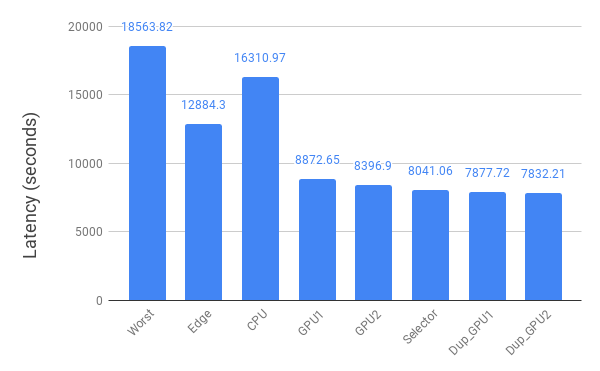
\includegraphics[scale=0.42]{latency.png}
%\caption{The Total Latency of the worst scenario, single runtimes, selector
%and duplicators. } \label{fig:latency} \end{figure}
%
%We next analyze the duplicator of edge cloud versus gpu2. According to the MDE
%metric, gpu2 runtime has more variable deployment and processing time compared
%to gpu1 runtime, which possibly leads to a lower success rate of selection.
%The analytics of the data proves this assumption that STOIC only makes right
%selection between edge cloud and gpu2 runtime by 94.8\% of times, 1.9\% lower
%than being with gpu1 runtime. However, as depicted in the
%Figure~\ref{fig:latency}, the total latency of single gpu2 runtime is shorter
%than the total latency for single gpu1 runtime. We argue that even though
%STOIC make slightly more mistakes in this mode, the duplicator of gpu2 forms a
%faster and more efficient dispatching system. Demonstrated in the
%Table~\ref{tab:comparison}, duplicator of gpu2 runtime achieves the lowest
%average latency (50.86 seconds) and highest speedup (2.37x). We plan to
%investigate runtimes with more GPUs and the trade-off between the
%predictability and efficiency of system as future work.

\iffalse
Table~\ref{tab:success} summarizes the possible success failure cases for the
Duplicator.
\begin{table}[t] 
\centering
\captionsetup{justification=centering}
\scriptsize
\resizebox{\columnwidth}{!}{
\begin{tabular}{|c|c|c|c|} 
\hline
\textbf{\makecell{Predicted GPU \\Lower Latency}} & \textbf{Switch to GPU} & \textbf{\makecell{Actual GPU \\Lower Latency} } & \textbf{Case Label}\\
\hline
Yes & Yes & Yes & Success \\
\hline
Yes & Yes & No & Success \\
\hline
Yes & No & Yes & \textbf{Failure} \\
\hline
Yes & No & No & Success \\
\hline
No & Yes & Yes & Success\\
\hline
No & Yes & No & Success \\
\hline
No & No & Yes & \textbf{Failure} \\
\hline
No & No & No & Success \\
\hline
\end{tabular}
}
\caption{
Duplicator success/failure cases for STOIC.}
\label{tab:success}
\end{table}

\begin{algorithm}[]
\caption{Duplicator Success Rate Heuristic}
\label{algo:optimizer}
\SetAlgoLined
\KwData{Executions on Edge and GPUx runtime}
\KwResult{Runtime Selection Labels}
\For{Executions on Edge and GPUx}{
 \eIf{Predicted GPUx $T_s$ $<$ Predicted Edge $T_s$}{
    \eIf{Predicted Edge $T_s$ - (Actual GPUs $T_t$ + Actual GPUs $T_d$)) $\ge$ Predicted GPUx $T_s$}{
    \eIf{Actual GPUx $T_s$ $<$ Actual Edge $T_s$}{SUCCESS}{SUCCESS}
 }{
    \eIf{Actual GPUx $T_s$ $<$ Actual Edge $T_s$}{FAILURE}{SUCCESS}}}
 {
 \eIf{Predicted Edge $T_s$ - (Actual GPUs $T_t$ + Actual GPUs $T_d$)) $\ge$ Predicted GPUx $T_s$}{
    \eIf{Actual GPUx $T_s$ $<$ Actual Edge $T_s$}{SUCCESS}{SUCCESS}
 }{
    \eIf{Acutal GPUx $T_s$ $<$ Actual Edge $T_s$}{FAILURE}{SUCCESS}}
 }
}
\end{algorithm}
\fi


\section{Related Work}
\label{sec:related}
We explored an early design and scheduler for STOIC in~\cite{ref:stoic2020}.  This paper extends this workshop paper with a new scheduling system and consideration of both individual and concurrent edge-cloud placements. Many great prior works~\cite{ref:lowlatency, ref:bandwidth, ref:MAUI}, which have explored low-latency geo-distributed data analytics and mobile-cloud offloading, inspires the architecture design of STOIC. Furthermore, this work focuses on IoT infrastructure leveraging serverless computing and GPUs on ecological application. Hence, we consider recent advances in machine learning infrastructure, serverless computing, GPU accelerators, and Kubernetes orchestration service. \cite{ref:serverlessstep} and \cite{ref:berkeleyserverless} conduct a comprehensive survey on serverless computing including challenges and research opportunities. We share the same viewpoint that the use of the serverless execution model will grow for online training and inference applications. \cite{ref:deepserving} provides a prototype for a deep learning model serving in a serverless platform. \cite{ref:accelerated} provides another use case for accelerating serverless functions by GPU virtualization in data centers. Unique in our work, STOIC extends an existing serverless framework to support GPU acceleration and distributed function placement across the edge and public clouds. \cite{ref:evaluation} evaluates several serverless frameworks based on Kubernetes. We also employ Kubernetes for container orchestration, which is lightweight, flexible, and developer-friendly.  We concur that Kubernetes is a promising deployment infrastructure for serverless computing.  

The second relevant domain of related work is image recognition on IoT devices and edge clouds. \cite{ref:face} compares the processing time of face recognition between the edge device and IoT, namely smartphones. It concludes that edge devices perform comparably faster and scales better as the number of images increases. We agree with this conclusion, and as such, design STOIC to offload image processing workloads to both edge clouds and public clouds. \cite{ref:DDNN} proposes a distributed deep neural network that allows fast and localized inference at the edge device using truncated layers of a neural network. \cite{ref:cooperative} defines edge cloud offloading as a Markov decision process (MDP) whose objective is to minimize the average processing time per job. Based on this setting, it provides a novel approximate solution to MDP with a one-step policy iteration. These works are complementary to STOIC and we are considering how to incorporate them into the system as part of future work.

Also complimentary to STOIC, are tracing, testing, repair, and profiling tools (which STOIC can leverage) for serverless systems. Multiple works track causal dependencies across distributed serverless deployments for use in optimization, placement, and data repair~\cite{ref:repairdata,deptracing19,gammaray17,aws-xray}. FaaSProfiler~\cite{ref:profile} provides a tool for testing and profiling STOIC as a FaaS platform. \cite{ref:security} proposes a security solution that applies reinforcement learning (RL) to provide secure offloading to the edge nodes to prevent jamming attacks. These related systems can be combined with STOIC to provide a robust serverless ecosystem for distributed IoT devices.



\section{Conclusion}
\label{sec:conc}
In this paper, we propose a framework, called STOIC, for executing machine learning applications in IoT-cloud settings using the serverless architecture. STO\-IC integrates an edge controller and a public cloud with GPU acceleration. When the scheduler at the edge controller receives a batch of images from open field camera traps, it predicts the total response time for processing the batch based on batch size and historical log data. In the selector mode, STOIC schedules the task to the runtime with the least predicted latency. In the duplicator mode, STOIC co-schedules the task on the edge cloud and GPU runtime in the public cloud. If the latter is deployed and predicted to be faster, the edge cloud job is terminated. Otherwise, STOIC terminates the public cloud job and completes the task on the edge cloud. This mode further optimizes the selection process by avoiding volatile deployment times.

We present the design principles, implementation details, the feedback control mechanism, and different modeling methodologies to address the variability in the edge and public cloud deployments. Our empirical evaluation demonstrates STOIC can schedule tasks on local and remote deployments to achieve a speedup of 3.3x versus our baseline scenario. STOIC's success rate for prediction placement  ranges from 92\% to 97\% for the application and datasets that we study. 

As part of future work, we plan to investigate substituting RANSAC with Gradient Boosting Regression Trees (GBRT) to capture the non-linearity in the processing time due to heterogeneous hardware across deployment options (runtimes). We also plan to investigate model check-pointing in duplicator mode to better utilize computational resource on edge cloud and to improve the overall performance of the STOIC system.


% cannot include this until paper is unblinded
%\section*{Acknowledgments}
%This work has been supported in part by NSF (CNS-1703560, CCF-1539586,
%ACI-1541215), ONR NEEC (N00174-16-C-0020),
%and the AWS Cloud Credits for Research program.
%This work was performed in part at the University of California Natural Reserve System Sedgwick Reserve DOI: 10.21973/N3C08R.




\bibliographystyle{ama}
\bibliography{ref_ama}

\end{document}


